\documentclass[a4paper, 12pt]{article}

\def\languages{french, english}

%%%%%%%%%%%%%%%%%%% Libraries

\input{./include/libraries/default.tex}
\input{./include/libraries/figures.tex}
\input{./include/libraries/mathematics.tex}
\input{./include/libraries/units.tex}

%%%%%%%%%%%%%%%%%%% Titlepage

\def\logopath{./resources/pdf/logo.pdf}
\def\toptitle{University of Liège}
\title{Project 1 - Exploratory data analysis}
\def\subtitle{\textsc{MATH2021-1} - High-dimensional data analysis}
%\def\authorhead{}
\author{
Yann \textsc{Claes} (s161317)\\
Gaspard \textsc{Lambrechts} (s161826)\\
François \textsc{Rozet} (s161024)\\
}
%\def\rightauthorhead{}
%\def\rightauthor{}
\def\context{MSc in Data science and engineering}
\date{Academic year 2019-2020}

%%%%%%%%%%%%%%%%%%%

\usepackage{mhchem}
\usepackage{wrapfig}
\usepackage{verbatim}

%%%%%%%%%%%%%%%%%%%

\begin{document}
	\input{include/titlepages/default.tex}
	\section{Data}
	The chosen data set describes the evolution of major air pollutants and meteorological variables in 12 air-quality monitoring stations of Beijing. The hourly measured data spread from March 1st, 2013 to February 28th, 2017. \par
	\subsection{Variables}
	The pollutants measured are the concentrations (\si{\micro\gram\per\meter\cubed}) of $\text{PM}_{2.5}$, $\text{PM}_{10}$\footnote{Particle matter of size up to $\SI{2.5}{}$, respectively, $\SI{10}{\micro\meter}$.}, $\ce{SO2}$, $\ce{NO2}$, $\ce{CO}$ and $\ce{O3}$. The meteorological variables are the temperature (\si{\degreeCelsius}), the pressure (\si{\hecto\pascal}), the dew point temperature (\si{\degreeCelsius}), the rain precipitation (\si{\milli\meter}) and the wind speed (\si{\meter\per\second}). The data set also features the wind direction as compass-like directions (N, S, W, NE, etc.). \par
	With the assigned index, the time described by four variables (year, month, day and hour) and the station name, each line of the data set presents 18 columns/variables including 11 continuous.
	\subsection{Data handling}
	First of all, in order to greatly reduce the data quantity, it has been decided to limit the analysis to the measurements of the \emph{Shunyi} station. Still, the number of rows/individuals in the data set (roughly \num{35000}) was much more important than asked. Therefore, it has been decided to sample randomly (and uniformly) \num{500} of them. However, for the sake of consistency, a \emph{seed} has been set such that the sample is the same at each execution. \par
	Secondly, text being hardly analyzable mathematically, the compass-like directions have been converted into angles (\si{\radian}).\footnote{Unfortunately, this representation opposes $0$ to $2\pi$ while they actually are equivalent. A possible way to correct that behaviour would have been to replace the angles by their $\sin$ and $\cos$ in the data set.} \par
	Thirdly, the assigned index was replaced by a more genuine measure of time : the unix time stamp (i.e. the total number of seconds since January 1st, 1970). \par
	Finally, as can be seen in the contingency table of \texttt{rain} (cf. Table \ref{tab:rain}), its continuous nature is quite disputable. \par
	\begin{table}[H]
	    \centering
	    \begin{tabular}{|c|c|c|c|c|}
	        \hline
	        \texttt{rain} $\sbk{\si{\milli\meter}}$ & \num{0} & \num{0.1} to \num{0.8} & \num{1} to \num{1.6} & \num{15} \\ \hline\hline
	        Occurrence & \num{483} & \num{12} & \num{4} & \num{1} \\ \hline
	    \end{tabular}
	    \noskipcaption{Contingency table of the variable \texttt{rain}.}
	    \label{tab:rain}
	\end{table}
	Indeed, it seems that the fact it has rained, whatever the quantity, is \emph{abnormal}. Based on that observation, \texttt{rain} has been transformed into a binary indicator : \texttt{FALSE} if it hasn't rained and \texttt{TRUE} if it has.
	\subsection{Scientific question}
	Air pollution in cities becomes more and more concerning, especially for children. This data set might help to predict pollution peaks and warn the population about it.
	\section{Missingness}
	Firstly, a plot displaying the global missingness of the selected data subset has been drawn using the \texttt{vis\_miss} function, resulting in Figure \ref{fig:vis_miss}. A total \num{1.8} percentage of missingness is observed. \par
	\begin{wrapfigure}{R}{0.55\textwidth}
	    \vspace{-2em}
	    \centering
	    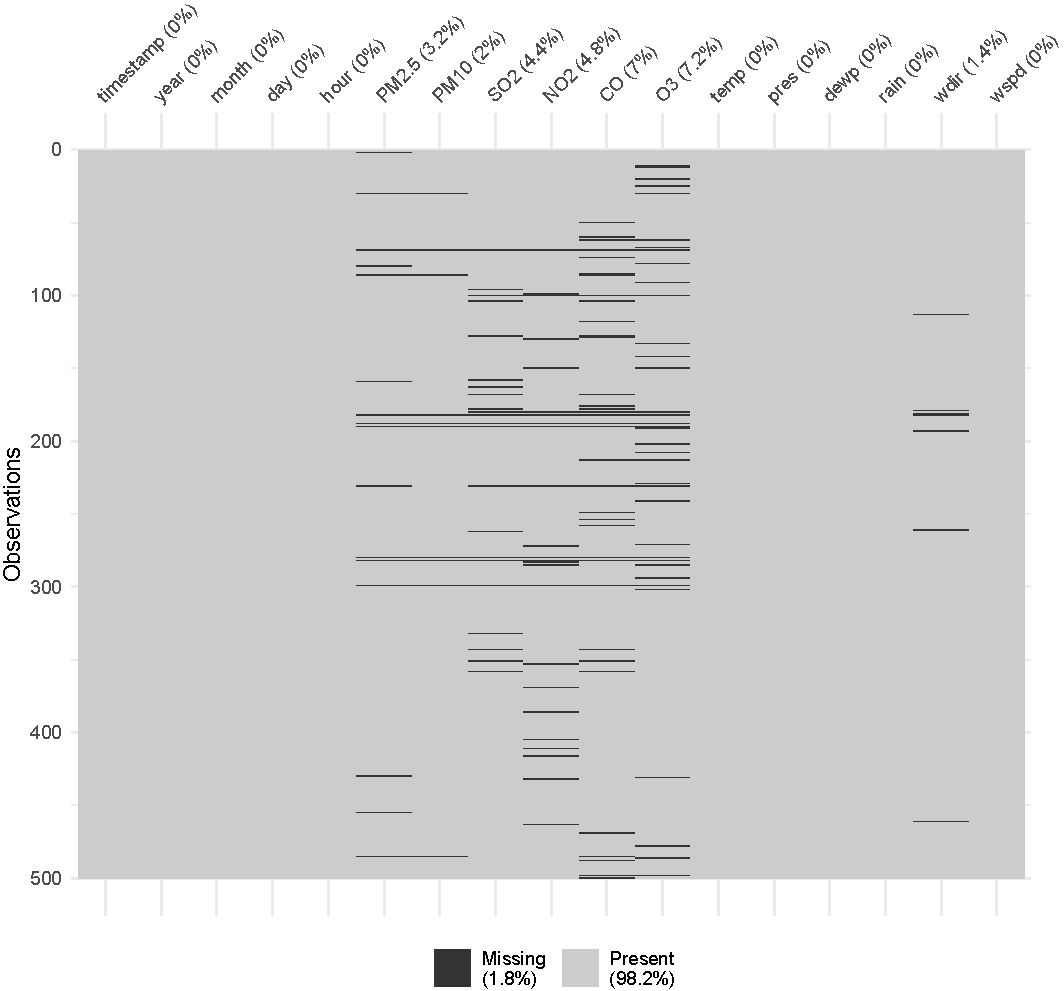
\includegraphics[width=0.54\textwidth]{resources/pdf/missingness_visualization.pdf}
	    \noskipcaption{Missingness in the data.}
	    \label{fig:vis_miss}
	    \vspace{-1em}
	\end{wrapfigure}
	The missing values are mostly present in the pollutant concentrations, while only a few of them are located in the \texttt{wdir} variable. \par
	To observe potential patterns between the missing variables, an upset plot has been derived using the \texttt{gg\_miss\_upset} function from the \texttt{naniar} library, leading to Figure \ref{fig:gg_miss_upset}. \par
	\begin{wrapfigure}{L}{0.55\textwidth}
	    \vspace{-1em}
	    \centering
	    \includegraphics[width=0.54\textwidth]{resources/pdf/missingness_patterns.pdf}
	    \noskipcaption{Upset plot of the missing data.}
	    \label{fig:gg_miss_upset}
	    \vspace{-1em}
	\end{wrapfigure}
    At first glance, no real pattern can be distinguished as most ($61$) cases involve variables individually. Only $7$ rows of the data set have missing values for all the pollutant concentrations. This could be the result of all sensors breaking down at the same time, due to unknown reasons, or of the central system failing to write the measurements to the database.
    \subsection{Missing data mechanism}
	In order to spot the potential reasons for which a variable could be missing, the following strategy has been used : for each pair of variables $X$ and $Y$ where $X$ has missing values, the z-score of the mean of $Y$ when $X$ is missing has been computed. This z-score gives an insight on the potential influence of the variable $Y$ on the missingness of $X$. \par
	Indeed, if the missingness of $X$ is independent of $Y$, $m^*$, the mean of the $n$ values of $Y$ for which $X$ is missing, should be an unbiased estimator of the actual mean of $Y$. Therefore, assuming that $Y$ is normal,
	\begin{equation*}
	    P\rbk{\frac{m^* - \mu}{\frac{\sigma}{\sqrt{n}}} \in \sbk{- u_{\frac{p}{2}}, u_{\frac{p}{2}}}} = 1 - p \, ,
	\end{equation*}
	i.e. the z-score of $m^*$ should belong to the confidence interval $\sbk{- u_{\frac{p}{2}}, u_{\frac{p}{2}} }$ with a probability $1 - p$, where $u_{x}$ is such that
	\begin{equation*}
	    P\rbk{\mathcal{Z} > u_{x}} = x, \quad \mathcal{Z} \sim \mathcal{N}(0, 1) \, .
	\end{equation*}
	For example, taking $1 - p$ as $95 \%$, the confidence interval becomes $\sbk{- \num{1.96}, \num{1.96} }$. \par
	\begin{wrapfigure}{R}{0.5\textwidth}
	    \vspace{-1em}
	    \centering
	    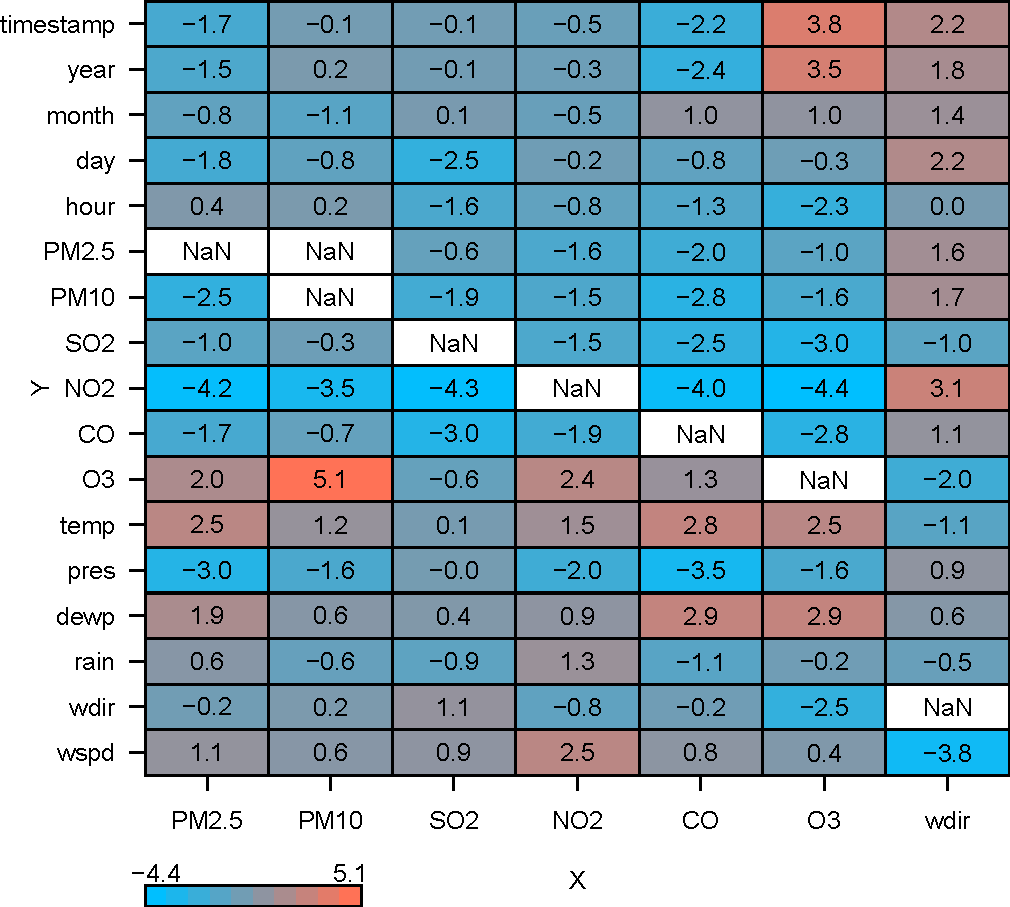
\includegraphics[width=0.49\textwidth]{resources/pdf/zs_mean_NA.pdf}
	    \noskipcaption{Z-score of the mean of $Y$ when $X$ is missing.}
	    \label{fig:z-scores}
	    \vspace{-2em}
	\end{wrapfigure}
	Therefore, high (or low) z-scores might be clues to relations between $Y$ and the missingness of $X$, but only if $Y$ follows a normal distribution. Unfortunately, it is not the case of any pollutants (cf. section \ref{sec:univariate_analysis}), which might explain such extremes scores one can see in Figure \ref{fig:z-scores}. \par
	Furthermore, if most variables present high value z-scores, only a few possible explanations could be drawn :
    \paragraph{Wind speed and direction} Although the wind speed does not follow a normal distribution, the observed z-score for $Y$ as the wind speed and $X$ as the wind direction is quite remarkable since a \num{-3.8} z-score is reserved to abnormally low values. Indeed, by looking at the boxplots drawn at Figure \ref{fig:wspd_wdir_missingness.pdf}, it could be deduced that missing values of wind direction are the logical results of a barely present wind, i.e. a wind whose speed is almost null.
    \begin{wrapfigure}{R}{0.5\textwidth}
        \vspace{-1em}
	    \centering
	    \includegraphics[width=0.49\textwidth]{resources/pdf/wspd_wdirmiss.pdf}
	    \noskipcaption{Wind speed boxplots according to the missingness of the wind direction.}
	    \label{fig:wspd_wdir_missingness.pdf}
	    \vspace{-0em}
    \end{wrapfigure}
    \paragraph{Temperature, dew point and pressure} As one can see in Figure \ref{fig:z-scores}, these three variables present multiple abnormal z-scores. If it is hardly possible to induce any direct link from that observation, it is however not risky to say there probably exists relations between the missingness of pollutants such as \ce{CO} and \ce{O3} and the temperature since temperature-caused troubleshoot are quite current. \par
    Furthermore, because of the linear correlation between temperature, dew point and pressure (cf. section \ref{sec:multivariate_analysis}) it is perfectly logic to observe such visible correlation between their z-scores.
	Eventually, it is not possible to conclude anything with certitude about the missing data mechanism. However, it seems almost certain that it is not \emph{MCAR} and \emph{MAR} seems to hold quite well to observations.
	\subsection{Dealing with missing data}
	For the exploratory part, it has been chosen to perform a \emph{complete case analysis}, i.e. to delete all rows containing missing data that is to remove \num{86} rows. This strategy ensures to analyze a data set without any statistical artefact like those unconditional or conditional imputations would inevitably introduce.
	\section{Exploratory analysis}
	\subsection{Univariate analysis} \label{sec:univariate_analysis}
	First of all, the univariate statistics, listed in Table \ref{tab:univariate_statistics}, of relevant variables have been computed using the \texttt{summary} function of \texttt{R}.
    \begin{table}[H]
        \centering
        \begin{tabular}{|c|c|c|c|c|c|c|c|c|c|c|c|}
            \cline{2-11}
            \multicolumn{1}{c|}{} & \texttt{PM2.5} & \texttt{PM10} & \texttt{NO2} & \texttt{SO2} & \texttt{CO} & \texttt{O3} & \texttt{temp} & \texttt{pres} & \texttt{dewp} & \texttt{wspd} \\ \hline
            Units & \multicolumn{6}{c|}{\si{\micro\gram\per\meter\cubed}} & \si{\degreeCelsius} & \si{\hecto\pascal} & \si{\degreeCelsius} & \si{\meter\per\second} \\ \hline\hline
            Min & \num{3.0} & \num{5.0} & \num{1.0} & \num{4.0} & \num{100} & \num{1.0} & \num{-13.6} & \num{991.7} & \num{-25.9} & \num{0} \\
            Median & \num{58.0} & \num{83.5} & \num{7.0} & \num{46.0} & \num{900} & \num{34.0} & \num{11.75} & \num{1014.1} & \num{0.35} & \num{1.5} \\
            Mean & \num{86.5} & \num{108.3} & \num{15.4} & \num{49.6} & \num{1295} & \num{49.8} & \num{11.6} & \num{1014.6} & \num{1.1} & \num{1.7} \\
            Max & \num{470.0} & \num{485.0} & \num{192.0} & \num{187.0} & \num{7000} & \num{293.0} & \num{37.9} & \num{1035.7} & \num{25.0} & \num{6.8} \\
            Std & \num{82.8} & \num{90.0} & \num{20.9} & \num{31.4} & \num{1148} & \num{54.4} & \num{11.2} & \num{9.9} & \num{13.1} & \num{1.15} \\ \hline
        \end{tabular}
        \noskipcaption{Univariate statistics summary.}
        \label{tab:univariate_statistics}
    \end{table}
    At first glance, one can notice that the median and mean of the pollutants are quite dissimilar while those of the temperature, pressure and dew point are pretty close. That observation is strengthened by the histograms in Figure \ref{fig:histograms}. Indeed, the pollutants do not seem to follow normal (nor symmetrical) distributions, while the temperature, pressure and dew point seem to. As far as the wind speed is concerned, it seems to follow a Poisson-like distribution.
	\subsection{Multivariate analysis} \label{sec:multivariate_analysis}
	\begin{wrapfigure}{r}{0.5\textwidth}
	    \vspace{-5em}
	    \centering
	    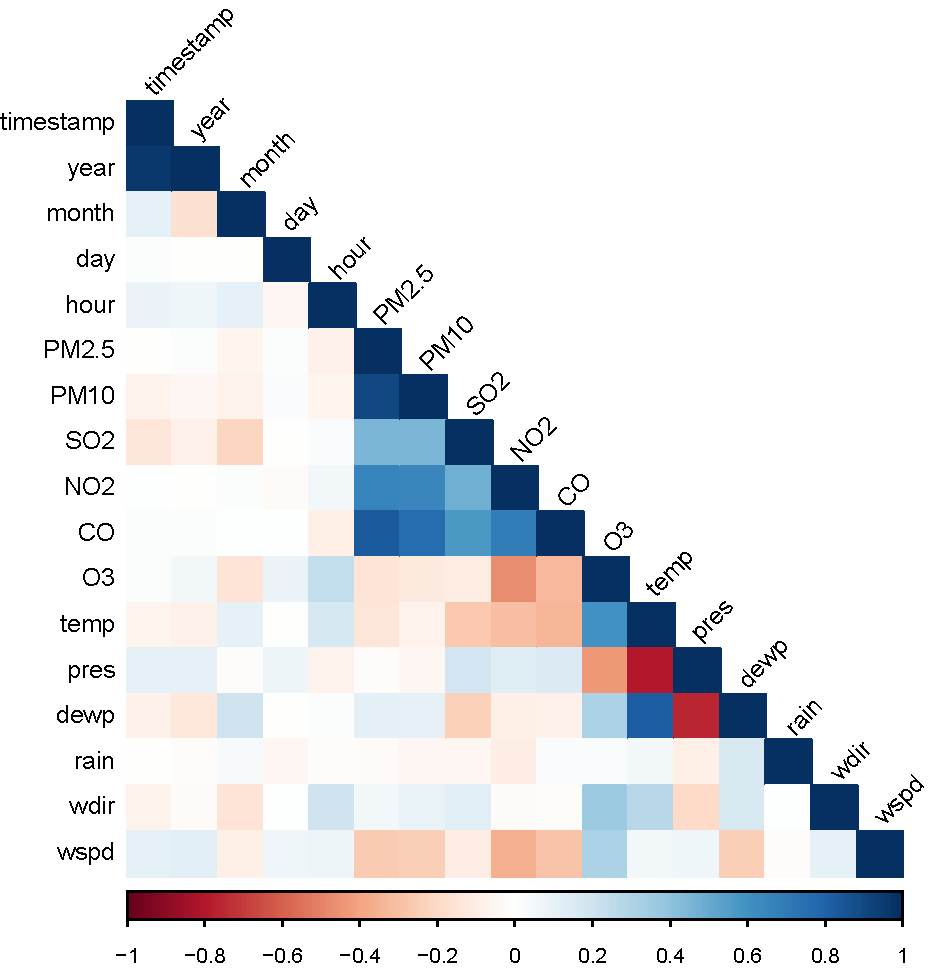
\includegraphics[width=0.48\textwidth]{resources/pdf/correlation.pdf}
	    \noskipcaption{Correlation plot of the variables.}
	    \label{fig:corrplot}
	    \vspace{-3em}
	\end{wrapfigure}
	In order to get an overall visualization of the potential correlation between some of the variables, a correlation plot has been derived. By sticking to this correlation only, non-linear dependencies between variables could be missed. These other dependencies will be discussed later. \par
	As one can see in Figure \ref{fig:corrplot}, there is a positive correlation between all the pollutant concentrations, except ozone (\ce{O3}). Indeed, the latter has little anti-correlation with the \ce{CO} concentration and stronger anti-correlation with the \ce{NO2} concentration. \par
	This \emph{anti}-correlation can be explained by the following chemical equilibrium :
	\begin{equation}\label{eq:NO2_O3}
	    \ce{NO2 + O2 + UV + Heat <=> NO + O3}
	\end{equation}
	This effect is even more visible on the scatter matrix of Figure \ref{fig:pairs_pollutants} (where only 100 rows have been sampled in order to make the plot readable). \par
	Also, the pollutant concentrations are slightly dependent on the temperature, especially for \ce{NO2} and \ce{O3}. As far as these two pollutants are concerned, it may be explained by the chemical equilibrium given above. This behaviour can be observed in Figure \ref{fig:pollutant_temp}\footnote{A locally estimated scatter plot smoothing estimator with confidence intervals for the conditional mean has been plotted in order to help the eye in seeing patterns in these scatter plots. A drawback about these smoothing curves is that they do not take continuity into account. Indeed, smoothing over a whole year should give a periodic curve.}. \par
	\begin{figure}[h]
        \begin{subfigure}{.49\textwidth}
            \centering
            \includegraphics[width=0.95\textwidth]{resources/pdf/pollutants_months.pdf}
            \caption{Pollutant concentrations over the year}
            \label{fig:pollutant_months}
            \vspace{0.5em}
        \end{subfigure}
        \begin{subfigure}{.49\textwidth}
            \centering
            \includegraphics[width=0.95\textwidth]{resources/pdf/pollutants_temp.pdf}
            \caption{Pollutant concentrations w.r.t. temperature}
            \label{fig:pollutant_temp}
            \vspace{0.5em}
        \end{subfigure}
        \begin{subfigure}{.49\textwidth}
            \centering
            \includegraphics[width=0.95\textwidth]{resources/pdf/pollutants_hour.pdf}
            \caption{Pollutant concentrations over the day}
            \label{fig:pollutant_hour}
        \end{subfigure}
        \begin{subfigure}{.49\textwidth}
            \centering
            \includegraphics[width=0.8\textwidth]{resources/pdf/temp_months.pdf}
            \caption{Temperature evolution over the year}
            \label{fig:temp_months}
        \end{subfigure}
        \noskipcaption{Relation between temperature, pollutant concentrations and time.}
        \label{fig:temp_pollutant_months}
    \end{figure}
    It could suggest that the temperature causes or avoids the apparition of some pollutants, but that could also be due to a confounding factor, such as the period of the year or the wind direction which are, indeed, correlated with the temperature and pollutants as one can observe in Figures \ref{fig:pollutant_months}, \ref{fig:temp_months} and \ref{fig:wind}. \par
    \begin{figure}[h]
        \begin{subfigure}{.48\textwidth}
          \centering
          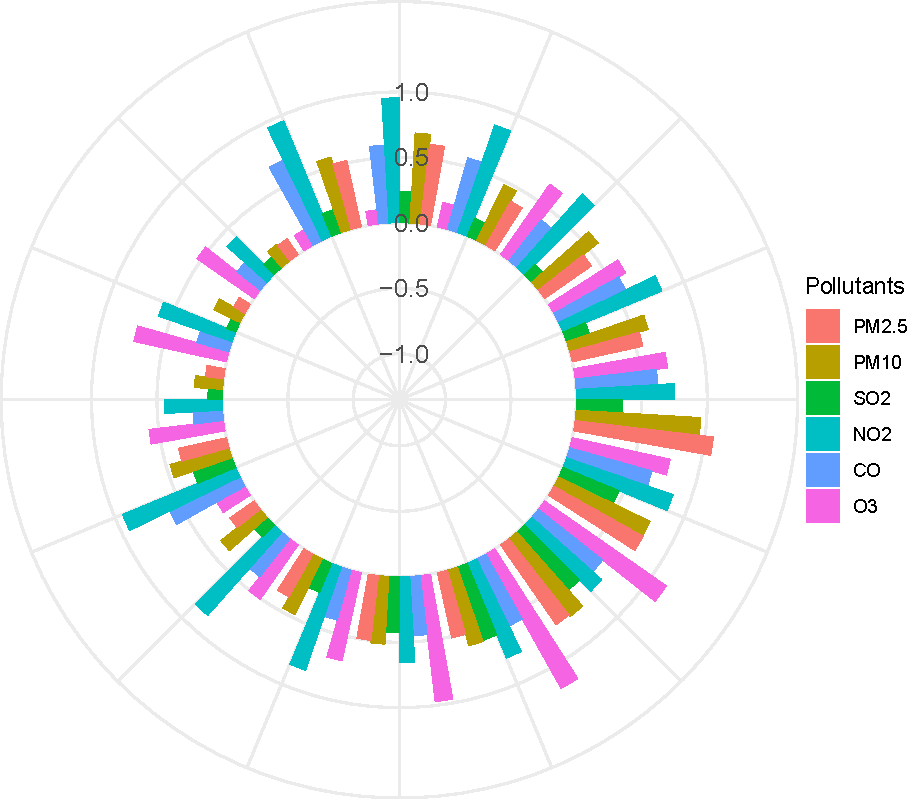
\includegraphics[height=0.9\textwidth]{resources/pdf/medianpollutants_wdir.pdf}
          \caption{Median pollutant concentrations w.r.t. wind direction}
          \label{fig:pollutants_wdir}
        \end{subfigure}
        \hspace{0.5em}
        \begin{subfigure}{.48\textwidth}
          \centering
          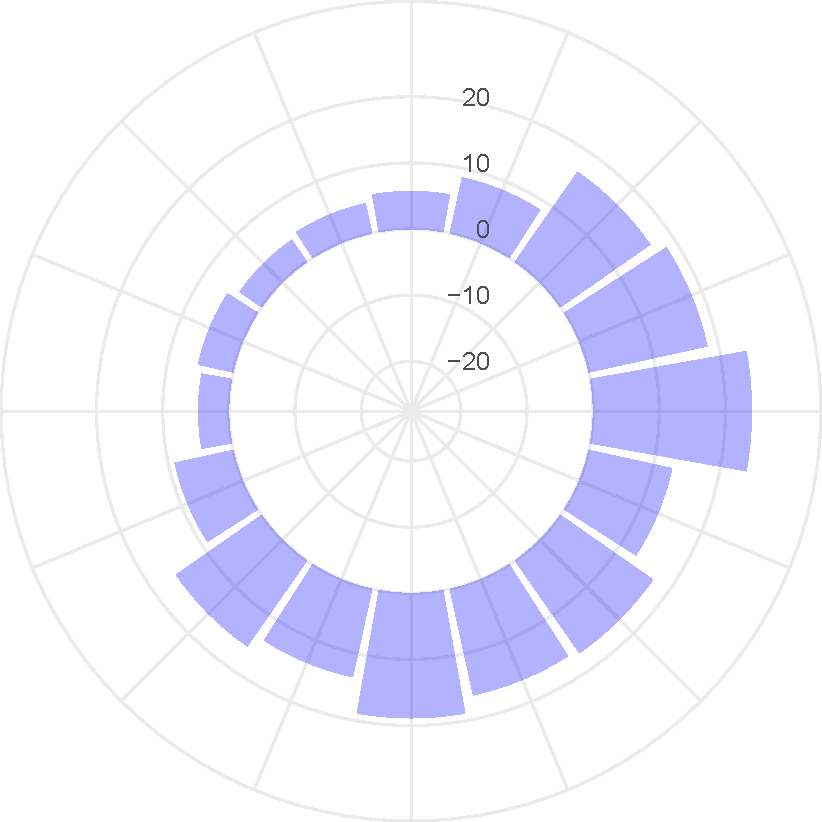
\includegraphics[height=0.9\textwidth]{resources/pdf/mediantemp_wdir.pdf}
          \caption{Median temperatures w.r.t. the wind direction}
          \label{fig:temp_dir}
        \end{subfigure}
        \noskipcaption{Circular plot of the temperature and pollutants w.r.t. the wind direction.}
        \label{fig:wind}
    \end{figure}
    \begin{comment}
    	From Figure \ref{fig:pollutant_months}, it can be seen that all pollutant concentrations follow the same curve, descending during the first half of the year, and ascending during the other half, except for the ozone concentration, which does the opposite. A plausible reason may be found in the chemical equilibrium above. Furthermore, by looking at Figure \ref{fig:temp_months}, one can observe that the temperature seems to follow a cosine trend over the year, ascending in the first half, descending in the second one. This behavior can be put in perspective with the previous Figure, emphasizing the relation between ozone, NO2 and high temperatures. Finally, taking a look at Figure \ref{fig:pollutant_temp} truly confirms the fact that the higher the temperature, the higher the concentration in ozone, and the lower the concentration in NO2. \par
        As can be seen from Figure \ref{fig:pollutants_wdir}, higher ozone concentrations seem to be linked with a South-East wind, while the other concentrations remain quite constant, except when the wind comes from the North-West, where they are rather small. By looking at Figure \ref{fig:temp_dir}, it can be noticed that higher temperatures are measured for South-East directions, while smaller ones are for North-West directions, emphasizing the equilibrium between temperature and O3-NO2 concentrations. \par
        However, the causality remains undetermined from these plots. Effectively, wind directions could influence temperatures, and thus influence pollutant concentrations, or vice versa.
    \end{comment}
    \begin{wrapfigure}{R}{0.55\textwidth}
	    \centering
	    \includegraphics[width=0.54\textwidth]{resources/pdf/pres_dewp_temp.pdf}
	    \noskipcaption{Evolution of the dew point with respect to temperature and pressure.}
	    \label{fig:pres_dewp}
	    \vspace{-4em}
	\end{wrapfigure}
	Another remarkable correlation is the one between the temperature and the dew point\footnote{The dew point is the minimum temperature to which air must be cooled in order to start condensing water vapor into liquid vapor.}. The dew point is strongly linearly correlated to the temperature. Actually, that relation is verified by the thermodynamic theory, since
	\begin{equation}\label{eq:dewp}
	    T_{dp} = T - \frac{100 - RH}{5}
	\end{equation}
	where $T_{dp}$ is the dew point, $T$ the temperature and $RH$ the relative humidity. \par
	Finally, the pressure is highly anti-correlated to the temperature, yet no convincing explanation could be found.
	\vspace{3em}
	\subsection{Qualitative analysis}
	As no qualitative variable could be found in the data set to conduct this analysis, it has been decided to analyze the impact of the binary indicator \texttt{rain} on the pollutant concentrations. This yielded the boxplots of Figure \ref{fig:pollutants_rain}. \par
	\begin{figure}[h]
	    \centering
	    \includegraphics[height=0.6\textwidth]{resources/pdf/pollutants_rain.pdf}
	    \noskipcaption{Effect of the rain on the concentrations of the different pollutants}
	    \label{fig:pollutants_rain}
	\end{figure}
	While some distributions might look different, for instance \ce{O3} and \ce{NO2}, hasty conclusions should not be drawn, as only \num{17} rows with positive precipitation are present in the data set. Indeed, there is no way of telling if both distributions would join or diverge if there were more rainy cases. \par
    \begin{comment}
    	Links can be made with respect to the correlation analysis discussed above. Effectively, the strong positive correlation between the PM2.5 and PM10 concentrations can be seen on the first two boxplots: when some rain is measured, both maximum concentrations drop compared to those when no rain is observed. In addition, the relationship between NO2 and O3 also fades on the corresponding boxplots: when rain is observed, the concentrations of NO2 are centered around 25 \si{\micro\gram\per\meter\cubed}, while those of O3 seem to increase, referring to the previous chemical equilibrium.
	\end{comment}
    For most atmospheric variables, the exact same conclusion should be drawn. However, the distribution of temperature and dew point are quite different in the dry and rainy cases. Indeed, Beijing's climate is a \emph{monsoon} climate which confirms the link between higher temperatures and rainy weather. Moreover, knowing equation \eqref{eq:dewp}, a rise of temperature and humidity should as well increase the dew point, as boxplots of Figure \ref{fig:atmospheric_rain} show.
	\begin{figure}[H]
	    \centering
	    \includegraphics[height=0.55\textwidth]{resources/pdf/atmospherical_rain.pdf}
	    \noskipcaption{Effect of the rain on the atmospheric variables}
	    \label{fig:atmospheric_rain}
	\end{figure}
	
	\subsection{Outlying observations}
    A plot gathering the z-score distributions for all the quantitative variables (except for the temporal ones) has been drawn, yielding Figure \ref{fig:z_scores_outlying}. From this plot, one can see that the assumed normal variables (i.e. \texttt{pres}, \texttt{temp}, \texttt{dewp}) do not seem to have outliers. This is not the case for the remaining variables, which do not follow normal distributions. \par
    \begin{figure}[h]
        \centering
        \includegraphics[height =     0.45\textwidth]{resources/pdf/z_scores.pdf}
        \noskipcaption{Z-score distributions}
        \label{fig:z_scores_outlying}
    \end{figure}
    The Mahalanobis distances have been computed through the \texttt{mahalanobis} function. Note that omitting the temporal variables may remove some dependencies between the variables, but this has been done to remain coherent with the z-score analysis done above. Results have been plotted in a bar plot, adding a line corresponding to the $95\%$ quantile of the chi-squared distribution, resulting in Figure \ref{fig:mahalanobis}. As most quantitative variables do not seem to follow normal distributions, interpretations should be relaxed with respect to the observed distances. Indeed, the number of outliers (\num{42}) is largely above $5 \%$ which confirms that pollutants do not follow normal distributions. \par
    \begin{figure}[h]
        \begin{subfigure}{.48\textwidth}
          \centering
          \includegraphics[height=0.9\textwidth]{resources/pdf/mahalanobis.pdf}
          \caption{Barplot}
          \label{fig:mahalanobis}
        \end{subfigure}
        \hspace{0.5em}
        \begin{subfigure}{.48\textwidth}
          \centering
          \includegraphics[height=0.9\textwidth]{resources/pdf/mahalanobis_boxplot.pdf}
          \caption{Boxplot}
          \label{fig:mahalanobis_boxplot}
        \end{subfigure}
        \noskipcaption{Mahalanobis distance plots.}
        \label{fig:wind}
    \end{figure}
    \newpage
    \appendix
    \section{Figures}
    \begin{figure}[h]
	    \centering
        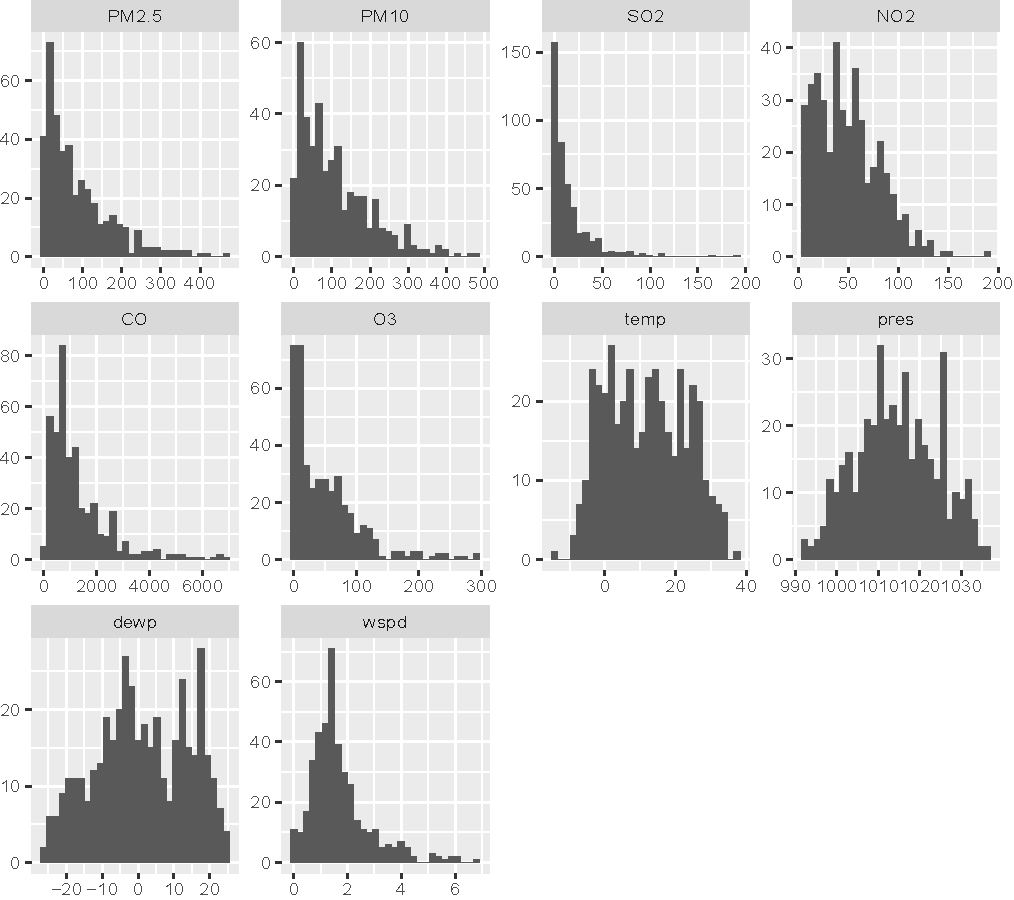
\includegraphics[width=0.9\linewidth]{resources/pdf/histograms.pdf}
        \noskipcaption{Histograms of the different variables.}
        \label{fig:histograms}
    \end{figure}
    \begin{figure}[h]
	    \centering
	    \includegraphics[width=0.9\textwidth]{resources/pdf/pairs_pollutants.pdf}
	    \caption{Scatter plots matrix of the different pollutant concentrations.}
	    \label{fig:pairs_pollutants}
	\end{figure}
\end{document}
